\documentclass[11pt,ngerman,a4paper]{article}
%Gummi|061|=)
\usepackage{amsmath}
\usepackage{a4wide}
\usepackage{amsthm}
\usepackage{amsbsy}
\usepackage{amssymb}
\usepackage{inputenc}
\usepackage{rotating} 
\usepackage{graphicx}
\usepackage{paralist}
\usepackage{selinput}
\SelectInputMappings{%
adieresis={ä},
germandbls={ß},
}
\title{\textbf{Versuch V351: Fourier Analyse und Synthese}}
\author{Martin Bieker\\
		Julian Surmann\\
		\\
		Durchgef\"{u}hrt am .01.2014\\
		Tu Dortmund}
\date{}
\usepackage{graphicx}
\begin{document}
\renewcommand\tablename{Tabelle}
\renewcommand\figurename{Abbildung}
\maketitle
\thispagestyle{empty}
\newpage
\clearpage
\setcounter{page}{1}


\section{Einleitung}

\section{Theorie}

\section{Vorbereitung und Durchf\"{u}hrung}
\subsection{Berechnung der Fouerierkoeffizienten}
Im Folgenden sollen die Fourierkomponenten von 3 verschiedenen Funktionen bestimmt werden. 
\paragraph{Dreicksfuntkion}
Die Dreiecksfuntkion ist definiert als
\begin{equation}
f \colon  \left[-\frac{T}{2}, \frac{T}{2}\right]\to \mathbb{R}, f(t) = 1 - \left|\frac{2t}{T}\right|
\end{equation}
Abbildung \ref{org_hut} zeigt die periodische Fortsetzung dieser Funktion.
\begin{figure}[htp]
\centering
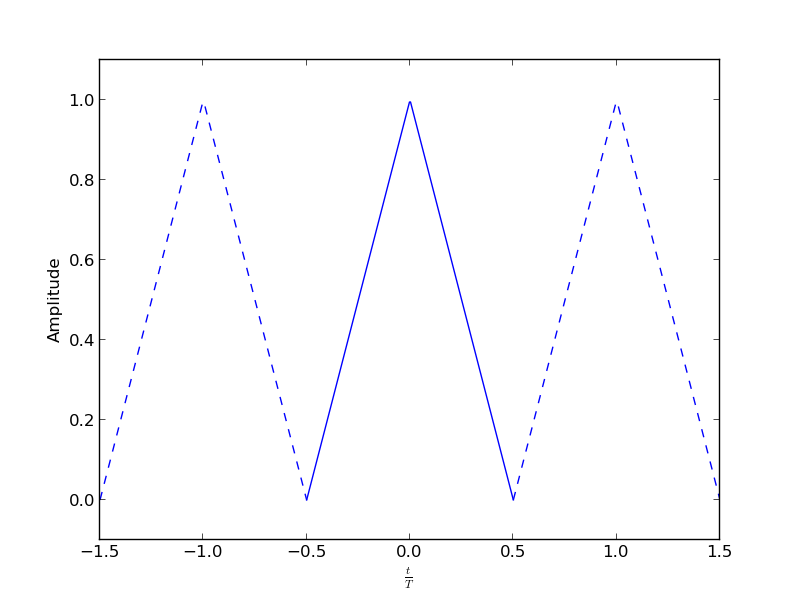
\includegraphics[scale=0.7]{abb/Abb2.png}
\caption{Periodische Fortsetzung der Dreicksfunktion}
\label{org_hut}
\end{figure} Da es sich bei dieser Abbildung um eine gerade Funktion handelt, sind alle Fourierkoeffizienten $b_n$ gleich null. Der Koeffizient $a_0$ betr\"agt nach Formel \ref{an}
\begin{equation} 
a_0 =\frac{2}{T} \int_{-\frac{T}{2}}^{\frac{T}2}\!f(t)\,\mathrm dt= \frac4T \int_{0}^{\frac{T}2}\!1-\frac{2t}{T}\,\mathrm dt= 1.
\end{equation}
F\"ur den Fall $n \neq 0$ folgt analog:
\begin{align}
a_n =\frac{2}{T} \int_{-\frac{T}{2}}^{\frac{T}2}\!f(t)cos\left(\frac{n2\pi t}{T}\right) \,\mathrm dt = \frac{4}{T} \int_0^\frac{T}2\!\left(1-\frac{2t}{T}\right)cos\left(\frac{n2\pi t}{T}\right)\,\mathrm dt \\= \frac{2 (1-(-1)^n)}{\pi^2n^2} = \begin{cases}
0 & n\mbox{ gerade} \\ \frac{4}{\pi^2n^2} & n\mbox{ ungerade}
\end{cases}
\end{align} 
\paragraph{S\"agezahnfunktion} Diese Abbildung ist durch
\begin{equation}
f \colon  \left[-\frac{T}{2}, \frac{T}{2}\right]\to \mathbb{R}, f(t) = t
\end{equation}
definiert. In Abbildung \ref{org_saw} ist die periodische Fortsetzung dieser Funktion zu sehen.
\begin{figure}[htp]
\centering
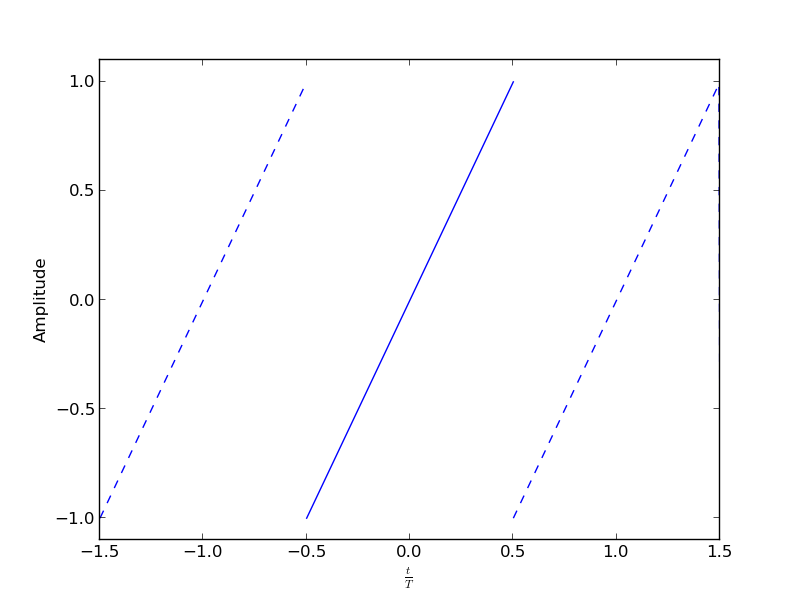
\includegraphics[scale=0.7]{abb/Abb1.png}
\caption{Periodische Fortsetzung der S\"agezahnfunktion}
\label{org_saw}
\end{figure} Da es sich bei dieser Funktion um eine ungerade Abbildung handelt, sind alle Koeffizienten $a_n$ gleich null. F\"ur die $b_n$ gilt nach Formel \ref{bn}:
\begin{align}
b_n = \frac 2 T\int_{-\frac T 2}^\frac T 2\!f(x)\,sin\left(\frac{n2\pi t}{T}\right)\,\mathrm dt = \frac 2 T \int_{-\frac T 2}^\frac T 2\!t\,sin\left(\frac{n2\pi t}{T}\right)\,\mathrm dt =\frac{ -2(-1)^n}{\pi n}\\=
\begin{cases}
-\frac{2}{\pi n} & n \mbox{ gerade}  \\
\frac{2}{\pi n} & n \mbox{ ungerade}
\end{cases}
\end{align}
\paragraph{Rechteckfuntion} Zur einfacheren Berechnung der Fourier-Koeffizienten wird diese Funtkion als
\begin{equation}
f \colon  \left[-\frac{T}{2}, \frac{T}{2}\right]\to \mathbb{R},\,f(t) = \begin{cases}
-1 & \mbox{f\"ur } n < 0 \\
1  & \mbox{f\"ur } n \geq 0
\end{cases}
\end{equation}
definiert. Die Abbildung \ref{org_rect} zeigt die periodische Fortsetzung dieser Funktion. 
\begin{figure}[htp]
\centering
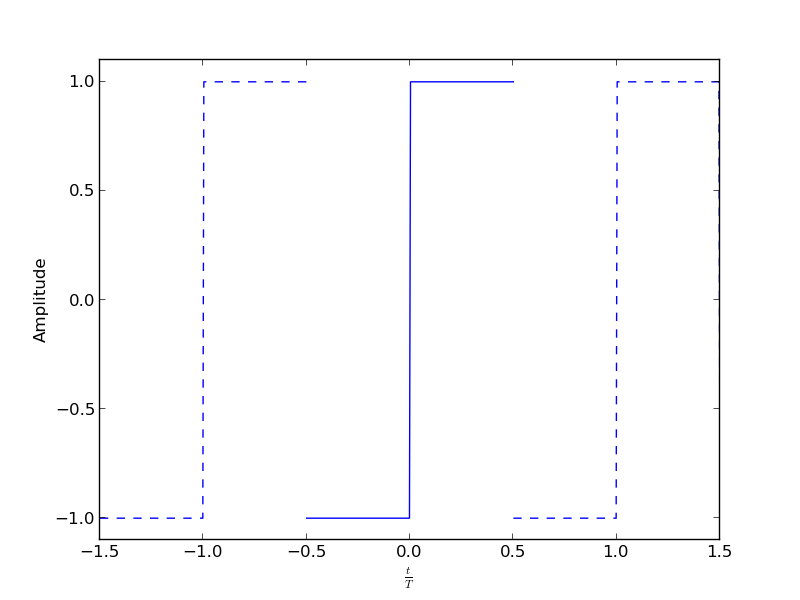
\includegraphics[scale=0.7]{abb/Abb3.png}
\caption{Periodische Fortsetzung der Rechteckfunktion}
\label{org_rect}
\end{figure}Da es sich auch bei dieser Funktion um eine ungerade Abbildung handelt sind analog zu oben alle $a_n$ gleich null. Des Weiteren sind die $b_n$ durch
\begin{align}
b_n = \frac 2 T\int_{-\frac T 2}^\frac T 2\!f(x)\,sin\left(\frac{n2\pi t}{T}\right)\,\mathrm dt = \frac 2 T \left[ \int_{-\frac T 2}^0\!sin\left(\frac{n2\pi t}{T}\right)\,\mathrm dt - \int_0^{\frac T 2}\!sin\left(\frac{n2\pi t}{T}\right)\,\mathrm dt \right] \\
= \frac{2 (1- (-1)^n)}{n \pi} =
\begin{cases}
0 & n \mbox{ gerade}\\
\frac4{n\pi} & n \mbox{ ungerade}
\end{cases} 
\end{align}
gegeben.
\subsection{Fourier-Analyse}
\subsection{Fourier-Synthese}
In diesem Versuchsteil sollen die verschiedenen Schwingungsformen aus ihren Fourier-Komponenten zusammengesetzt werden. Dazu wird ein so genannter Oberwellengenerator verwendet. Dies ist ein Ger\"at welches Sinusschwingungen mit festen Phasenbeziehungen und ganzzahligen Frequenzverh\"altnissen erzeugt. Zun\"achst werden dazu die Fourier-Keffizienten f\"ur die ersten 9 Oberwellen berechnet. Die Ergenisse finden sich in Tabelle \ref{koeff}.

\section{Auswertung}

\section{Diskussion}
\section{Abbildungsverzeichnis}
\section{Anhang}
\begin{itemize}
\item Tabellen
\item Auszug aus dem Messheft
\end{itemize}

\newpage
\begin{table}
\centering
\begin{tabular}{|c|c|c|c|}

\hline
n & Dreick [$a_n]$ & S\"agezahn [$b_n$] & Rechteck $[b_n]$ \\
\hline
1 & 0.405 & 0.637 & 1.273\\
2 & 0.0 & -0.318 & 0.0\\
3 & 0.045 & 0.212 & 0.424\\
4 & 0.0 & -0.159 & 0.0\\
5 & 0.016 & 0.127 & 0.255\\
6 & 0.0 & -0.106 & 0.0\\
7 & 0.008 & 0.091 & 0.182\\
8 & 0.0 & -0.08 & 0.0\\
9 & 0.005 & 0.071 & 0.141\\
\hline
\end{tabular}
\label{koeff}
\caption{Fourier-Koeffizienten der verschiedenen Schwingungen}
\end{table}
\end{document}